% Options for packages loaded elsewhere
\PassOptionsToPackage{unicode}{hyperref}
\PassOptionsToPackage{hyphens}{url}
%
\documentclass[
]{article}
\usepackage{lmodern}
\usepackage{amssymb,amsmath}
\usepackage{ifxetex,ifluatex}
\ifnum 0\ifxetex 1\fi\ifluatex 1\fi=0 % if pdftex
  \usepackage[T1]{fontenc}
  \usepackage[utf8]{inputenc}
  \usepackage{textcomp} % provide euro and other symbols
\else % if luatex or xetex
  \usepackage{unicode-math}
  \defaultfontfeatures{Scale=MatchLowercase}
  \defaultfontfeatures[\rmfamily]{Ligatures=TeX,Scale=1}
\fi
% Use upquote if available, for straight quotes in verbatim environments
\IfFileExists{upquote.sty}{\usepackage{upquote}}{}
\IfFileExists{microtype.sty}{% use microtype if available
  \usepackage[]{microtype}
  \UseMicrotypeSet[protrusion]{basicmath} % disable protrusion for tt fonts
}{}
\makeatletter
\@ifundefined{KOMAClassName}{% if non-KOMA class
  \IfFileExists{parskip.sty}{%
    \usepackage{parskip}
  }{% else
    \setlength{\parindent}{0pt}
    \setlength{\parskip}{6pt plus 2pt minus 1pt}}
}{% if KOMA class
  \KOMAoptions{parskip=half}}
\makeatother
\usepackage{xcolor}
\IfFileExists{xurl.sty}{\usepackage{xurl}}{} % add URL line breaks if available
\IfFileExists{bookmark.sty}{\usepackage{bookmark}}{\usepackage{hyperref}}
\hypersetup{
  pdftitle={Patterns of performance degradation during sleep restriction of long distance truck drivers},
  hidelinks,
  pdfcreator={LaTeX via pandoc}}
\urlstyle{same} % disable monospaced font for URLs
\usepackage[margin=1in]{geometry}
\usepackage{longtable,booktabs}
% Correct order of tables after \paragraph or \subparagraph
\usepackage{etoolbox}
\makeatletter
\patchcmd\longtable{\par}{\if@noskipsec\mbox{}\fi\par}{}{}
\makeatother
% Allow footnotes in longtable head/foot
\IfFileExists{footnotehyper.sty}{\usepackage{footnotehyper}}{\usepackage{footnote}}
\makesavenoteenv{longtable}
\usepackage{graphicx,grffile}
\makeatletter
\def\maxwidth{\ifdim\Gin@nat@width>\linewidth\linewidth\else\Gin@nat@width\fi}
\def\maxheight{\ifdim\Gin@nat@height>\textheight\textheight\else\Gin@nat@height\fi}
\makeatother
% Scale images if necessary, so that they will not overflow the page
% margins by default, and it is still possible to overwrite the defaults
% using explicit options in \includegraphics[width, height, ...]{}
\setkeys{Gin}{width=\maxwidth,height=\maxheight,keepaspectratio}
% Set default figure placement to htbp
\makeatletter
\def\fps@figure{htbp}
\makeatother
\setlength{\emergencystretch}{3em} % prevent overfull lines
\providecommand{\tightlist}{%
  \setlength{\itemsep}{0pt}\setlength{\parskip}{0pt}}
\setcounter{secnumdepth}{-\maxdimen} % remove section numbering

\title{Patterns of performance degradation during sleep restriction of long
distance truck drivers}
\author{}
\date{\vspace{-2.5em}}

\begin{document}
\maketitle

\hypertarget{presentation-of-the-case-study}{%
\subsection{Presentation of the case
study}\label{presentation-of-the-case-study}}

We are analysing the effect of sleep deprivation on reaction time of
long distance truck drivers. There are 18 subjects in the dataset and
for each subject, the reaction time was measured for 10 days. The
subjects were allowed only a limited amount of sleep for these 10
subsequent days. Each subject's reaction time was measured several times
on each day of the trial and an average was taken.

Reaction time is measured with a psychomotor vigilance task (PVT), which
measures the speed with which subjects respond to a visual stimulus.

Is there any relation between reaction time and the number of days of
sleep deprivation?

\hypertarget{exploratory-analysis}{%
\subsection{Exploratory analysis}\label{exploratory-analysis}}

\begin{verbatim}
##    Reaction Days Subject
## 1  249.5600    0     308
## 2  258.7047    1     308
## 3  250.8006    2     308
## 4  321.4398    3     308
## 5  356.8519    4     308
## 6  414.6901    5     308
## 7  382.2038    6     308
## 8  290.1486    7     308
## 9  430.5853    8     308
## 10 466.3535    9     308
## 11 222.7339    0     309
## 12 205.2658    1     309
\end{verbatim}

This dataset contains multiple measurements for each subject on
consecutive days, with as response variable the continuous variable
reaction time and explanatory variable Days. Since there are 10
measurements for each subject, it is a longitudinal study. The dataset
of 18 subjects is balanced with an equal amount of measurements for each
subject.

\hypertarget{spaghetti-plot}{%
\subsubsection{Spaghetti Plot}\label{spaghetti-plot}}

To visualise the individual reaction times and how they compare to the
mean, a spaghetti plot was created. This revealed that there was a
variation in intercepts or starting reaction times on day 0 between
subjects. This variation increased with subsequent days.

--\textgreater{} what is meant by variation? shouldnt we define it as
the difference between the minimum and maximum??

For most subjects, the reaction time increased with the amount of days
of sleep deprivation. This increase is also visible in the mean.

\textbackslash begin\{center\}\textbackslash includegraphics{[}width=0.8\linewidth,height=60\%
{]}\{Common\_sleep\_files/figure-latex/spaghetti-1\}
\textbackslash end\{center\}

\hypertarget{boxplot}{%
\subsection{Boxplot}\label{boxplot}}

The following boxplot was created to get a quick summary of the
dataset's characteristics. The mean and median seem to show a similar
increase throughout the study. For day nr 6, 7 and 10, outliers are
observed.\\
The variance increases with an increase in days of sleep deprivation but
the interquartile range appears to expand not as strongly as the minimum
and maximum of the boxplot.

To put together, some subjects deviate more from the mean with an
increase in days of sleep deprivation (see outliers on both sides) while
most others stay around the mean (see slower increase in interquartile
range).

The violin plot supports the above observations of the distribution of
the data around the mean with outliers.

\begin{center}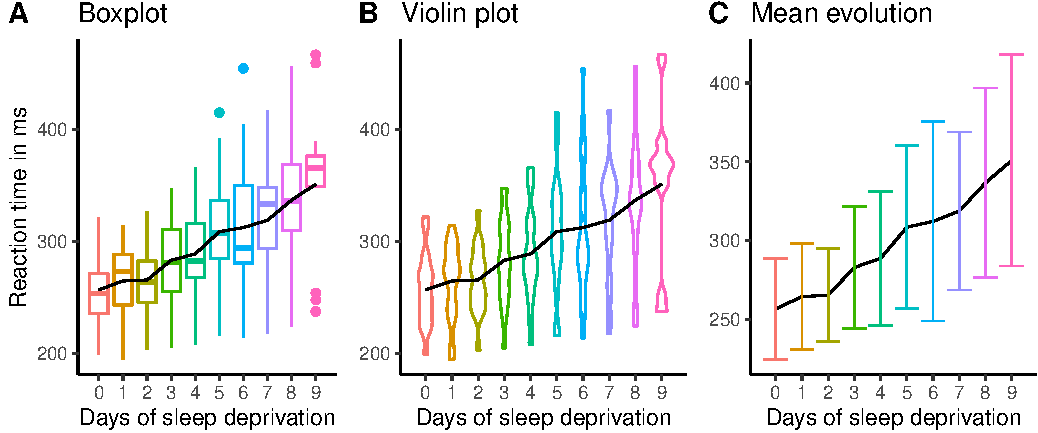
\includegraphics[width=0.8\linewidth]{Common_sleep_files/figure-latex/boxplot-1} \end{center}

\hypertarget{summary}{%
\subsection{Summary}\label{summary}}

\begin{longtable}[]{@{}lrrrrr@{}}
\toprule
& Days & Mean & SD & Var & n\tabularnewline
\midrule
\endhead
0 & 0 & 256.65 & 32.13 & 1032.30 & 18\tabularnewline
1 & 1 & 264.50 & 33.43 & 1117.59 & 18\tabularnewline
2 & 2 & 265.36 & 29.47 & 868.68 & 18\tabularnewline
3 & 3 & 282.99 & 38.86 & 1509.92 & 18\tabularnewline
4 & 4 & 288.65 & 42.54 & 1809.47 & 18\tabularnewline
5 & 5 & 308.52 & 51.77 & 2680.09 & 18\tabularnewline
6 & 6 & 312.18 & 63.17 & 3990.92 & 18\tabularnewline
7 & 7 & 318.75 & 50.10 & 2510.41 & 18\tabularnewline
8 & 8 & 336.63 & 60.20 & 3624.01 & 18\tabularnewline
9 & 9 & 350.85 & 66.99 & 4487.15 & 18\tabularnewline
The c & alculat & ions of t & he mean, & standard & deviation and
variance of the reaction time for each day of all subjects, further
support our exploratory plots: we observe an increase in the mean and
variance with more days of sleep deprivation.\tabularnewline
\bottomrule
\end{longtable}

\hypertarget{mean-evolution}{%
\subsection{Mean evolution}\label{mean-evolution}}

\begin{center}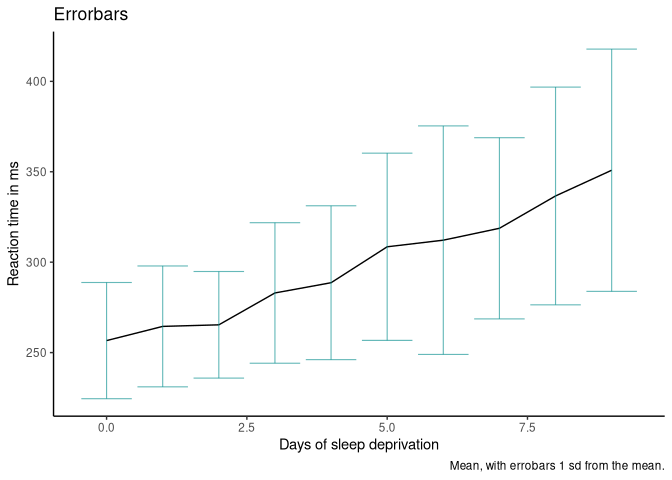
\includegraphics[width=0.8\linewidth]{Common_sleep_files/figure-latex/mean_err-1} \end{center}

To further support our previous findings, we looked at the mean
evolution. Here, an increasing trend of reaction time with increasing
number of days is also observed, together with expanding standard
deviations (see errorbars).

--\textgreater{} should we add anything more to this??

\hypertarget{correlation}{%
\subsection{Correlation}\label{correlation}}

\begin{longtable}[]{@{}lrrrrrrrrrrr@{}}
\toprule
& Subject & Reaction.0 & Reaction.1 & Reaction.2 & Reaction.3 &
Reaction.4 & Reaction.5 & Reaction.6 & Reaction.7 & Reaction.8 &
Reaction.9\tabularnewline
\midrule
\endhead
1 & 308 & 249.5600 & 258.7047 & 250.8006 & 321.4398 & 356.8519 &
414.6901 & 382.2038 & 290.1486 & 430.5853 & 466.3535\tabularnewline
11 & 309 & 222.7339 & 205.2658 & 202.9778 & 204.7070 & 207.7161 &
215.9618 & 213.6303 & 217.7272 & 224.2957 & 237.3142\tabularnewline
21 & 310 & 199.0539 & 194.3322 & 234.3200 & 232.8416 & 229.3074 &
220.4579 & 235.4208 & 255.7511 & 261.0125 & 247.5153\tabularnewline
31 & 330 & 321.5426 & 300.4002 & 283.8565 & 285.1330 & 285.7973 &
297.5855 & 280.2396 & 318.2613 & 305.3495 & 354.0487\tabularnewline
41 & 331 & 287.6079 & 285.0000 & 301.8206 & 320.1153 & 316.2773 &
293.3187 & 290.0750 & 334.8177 & 293.7469 & 371.5811\tabularnewline
51 & 332 & 234.8606 & 242.8118 & 272.9613 & 309.7688 & 317.4629 &
309.9976 & 454.1619 & 346.8311 & 330.3003 & 253.8644\tabularnewline
61 & 333 & 283.8424 & 289.5550 & 276.7693 & 299.8097 & 297.1710 &
338.1665 & 332.0265 & 348.8399 & 333.3600 & 362.0428\tabularnewline
71 & 334 & 265.4731 & 276.2012 & 243.3647 & 254.6723 & 279.0244 &
284.1912 & 305.5248 & 331.5229 & 335.7469 & 377.2990\tabularnewline
81 & 335 & 241.6083 & 273.9472 & 254.4907 & 270.8021 & 251.4519 &
254.6362 & 245.4523 & 235.3110 & 235.7541 & 237.2466\tabularnewline
91 & 337 & 312.3666 & 313.8058 & 291.6112 & 346.1222 & 365.7324 &
391.8385 & 404.2601 & 416.6923 & 455.8643 & 458.9167\tabularnewline
101 & 349 & 236.1032 & 230.3167 & 238.9256 & 254.9220 & 250.7103 &
269.7744 & 281.5648 & 308.1020 & 336.2806 & 351.6451\tabularnewline
111 & 350 & 256.2968 & 243.4543 & 256.2046 & 255.5271 & 268.9165 &
329.7247 & 379.4445 & 362.9184 & 394.4872 & 389.0527\tabularnewline
121 & 351 & 250.5265 & 300.0576 & 269.8939 & 280.5891 & 271.8274 &
304.6336 & 287.7466 & 266.5955 & 321.5418 & 347.5655\tabularnewline
131 & 352 & 221.6771 & 298.1939 & 326.8785 & 346.8555 & 348.7402 &
352.8287 & 354.4266 & 360.4326 & 375.6406 & 388.5417\tabularnewline
141 & 369 & 271.9235 & 268.4369 & 257.2424 & 277.6566 & 314.8222 &
317.2135 & 298.1353 & 348.1229 & 340.2800 & 366.5131\tabularnewline
151 & 370 & 225.2640 & 234.5235 & 238.9008 & 240.4730 & 267.5373 &
344.1937 & 281.1481 & 347.5855 & 365.1630 & 372.2288\tabularnewline
161 & 371 & 269.8804 & 272.4428 & 277.8989 & 281.7895 & 279.1705 &
284.5120 & 259.2658 & 304.6306 & 350.7807 & 369.4692\tabularnewline
171 & 372 & 269.4117 & 273.4740 & 297.5968 & 310.6316 & 287.1726 &
329.6076 & 334.4818 & 343.2199 & 369.1417 & 364.1236\tabularnewline
\bottomrule
\end{longtable}

\begin{verbatim}
## 
##  Shapiro-Wilk normality test
## 
## data:  sleep.resh[, i]
## W = 0.97667, p-value = 0.9093
## 
## 
##  Shapiro-Wilk normality test
## 
## data:  sleep.resh[, i]
## W = 0.94756, p-value = 0.388
## 
## 
##  Shapiro-Wilk normality test
## 
## data:  sleep.resh[, i]
## W = 0.98688, p-value = 0.9936
## 
## 
##  Shapiro-Wilk normality test
## 
## data:  sleep.resh[, i]
## W = 0.97738, p-value = 0.919
## 
## 
##  Shapiro-Wilk normality test
## 
## data:  sleep.resh[, i]
## W = 0.97247, p-value = 0.8427
## 
## 
##  Shapiro-Wilk normality test
## 
## data:  sleep.resh[, i]
## W = 0.978, p-value = 0.9271
## 
## 
##  Shapiro-Wilk normality test
## 
## data:  sleep.resh[, i]
## W = 0.95912, p-value = 0.5847
## 
## 
##  Shapiro-Wilk normality test
## 
## data:  sleep.resh[, i]
## W = 0.94648, p-value = 0.3724
## 
## 
##  Shapiro-Wilk normality test
## 
## data:  sleep.resh[, i]
## W = 0.97112, p-value = 0.8186
## 
## 
##  Shapiro-Wilk normality test
## 
## data:  sleep.resh[, i]
## W = 0.86251, p-value = 0.01342
\end{verbatim}

\begin{verbatim}
##            Reaction.0 Reaction.1 Reaction.2 Reaction.3 Reaction.4
## Reaction.0  1.0000000  0.6594427  0.5686275  0.4179567  0.4571723
## Reaction.1  0.6594427  1.0000000  0.7461300  0.6367389  0.5562436
## Reaction.2  0.5686275  0.7461300  1.0000000  0.8534572  0.7234262
## Reaction.3  0.4179567  0.6367389  0.8534572  1.0000000  0.9133127
## Reaction.4  0.4571723  0.5562436  0.7234262  0.9133127  1.0000000
## Reaction.5  0.2239422  0.3581011  0.4344685  0.6553148  0.7296182
## Reaction.6  0.2218782  0.2920537  0.4551084  0.6759546  0.7812178
## Reaction.7  0.3457172  0.3312693  0.5087719  0.4509804  0.5789474
## Reaction.8  0.1640867  0.1496388  0.2899897  0.4654283  0.5376677
## Reaction.9  0.3106295  0.2899897  0.3168215  0.4633643  0.5933953
##            Reaction.5 Reaction.6 Reaction.7 Reaction.8 Reaction.9
## Reaction.0  0.2239422  0.2218782  0.3457172  0.1640867  0.3106295
## Reaction.1  0.3581011  0.2920537  0.3312693  0.1496388  0.2899897
## Reaction.2  0.4344685  0.4551084  0.5087719  0.2899897  0.3168215
## Reaction.3  0.6553148  0.6759546  0.4509804  0.4654283  0.4633643
## Reaction.4  0.7296182  0.7812178  0.5789474  0.5376677  0.5933953
## Reaction.5  1.0000000  0.7667699  0.7254902  0.8121775  0.7378741
## Reaction.6  0.7667699  1.0000000  0.7110423  0.6904025  0.6181631
## Reaction.7  0.7254902  0.7110423  1.0000000  0.6573787  0.6243550
## Reaction.8  0.8121775  0.6904025  0.6573787  1.0000000  0.8452012
## Reaction.9  0.7378741  0.6181631  0.6243550  0.8452012  1.0000000
\end{verbatim}

\begin{center}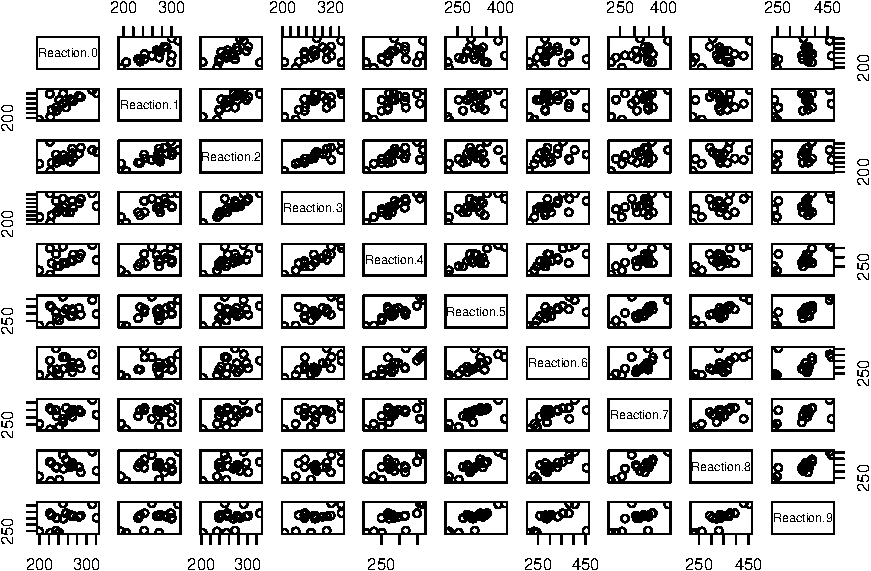
\includegraphics[width=0.8\linewidth]{Common_sleep_files/figure-latex/spearman-1} \end{center}

We used the Shapiro-Wilk test to check for normality of the reaction
times per day.

The test revealed a non normal distribution of day 9. Thus, we performed
the spearman correlation method instead of pearson to check for a
correlation of the reaction times between days.

--\textgreater{} is this correct?

Looking at the correlation matrix, there is a correlation higher then
0.6 between subsequent days (e.g.~between Day 8 and 9, between Day 3 and
4, \ldots). However, the further the days are apart, the lower the
correlation (e.g.~low correlation between Day 1 and Day 8).

Aligning nicely with our previous results, there is a linear trend
between the number of Days and reaction time. --\textgreater{} isn't
this another point?

\hypertarget{regression-per-person}{%
\subsection{Regression per person}\label{regression-per-person}}

\begin{center}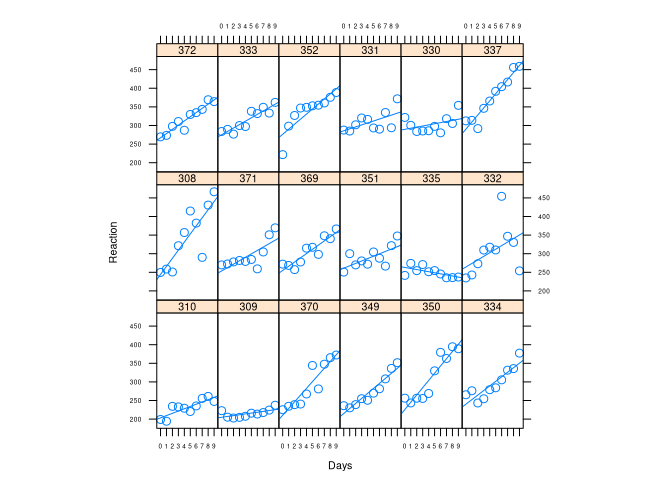
\includegraphics[width=0.8\linewidth]{Common_sleep_files/figure-latex/trellis-1} \end{center}

We performed a linear regression model on each subject based on the
function: reaction time = b0 + bi* Days.

We then created a trellis graph to visualise the intercepts and slopes
of these subject-specific linear regression models.

The graph suggests that the slope and intercept of each subject's linear
model are independent of each other as there is no observable trend
between the height of the intercept and the steepness of the slope.
Overall, all subjects have a positive slope besides subject 335.

The linear regression lines fit the datapoints closely, suggesting that
a linear model is appropriate to represent this dataset.

TO DISCUSS: correlation between slope/intercept?

\hypertarget{between-subject-variability}{%
\subsection{Between subject
variability}\label{between-subject-variability}}

\begin{center}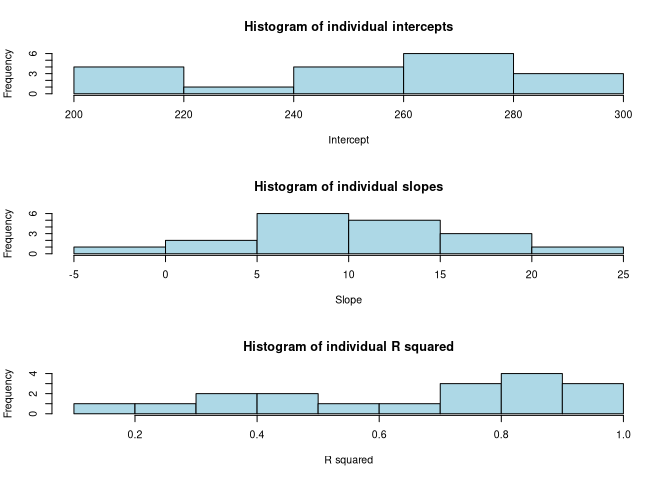
\includegraphics[width=0.8\linewidth]{Common_sleep_files/figure-latex/histograms-1} \end{center}

The individual intercepts shown in the first histogram correspond to the
initial reaction time and are non normally distributed. Given the small
data set, this is not surprising as it shows a variety of their initial
reaction time. However, if this data came from a large dataset, it would
be surprising that even the initial data points are not normally
distributed and could suggest a wrong data sample compared to the
population.

Looking at the histogram of individual slopes, we see a normal
distribution. As seen on the previous graph showcasing the individual
linear regressions, very little slopes are negative. This shows again
that reaction time increases by days of sleep deprivation.

Finally, looking at the histogram of R squared, we see that the majority
of subjects have a R squared of above 0.6. This shows that the linear
model is appropriate for this data set. However, sometimes the
individual linear model does not fit the specific data of some subjects,
specifically 7 of the 18 subjects.

\hypertarget{fitting-the-model---with-reml}{%
\subsection{Fitting the model - with
REML}\label{fitting-the-model---with-reml}}

\begin{verbatim}
## Linear mixed model fit by REML ['lmerMod']
## Formula: Reaction ~ 1 + Days + (1 + Days | Subject)
##    Data: sleep
## 
## REML criterion at convergence: 1743.6
## 
## Scaled residuals: 
##     Min      1Q  Median      3Q     Max 
## -3.9536 -0.4634  0.0231  0.4633  5.1793 
## 
## Random effects:
##  Groups   Name        Variance Std.Dev. Corr
##  Subject  (Intercept) 611.90   24.737       
##           Days         35.08    5.923   0.07
##  Residual             654.94   25.592       
## Number of obs: 180, groups:  Subject, 18
## 
## Fixed effects:
##             Estimate Std. Error t value
## (Intercept)  251.405      6.824  36.843
## Days          10.467      1.546   6.771
## 
## Correlation of Fixed Effects:
##      (Intr)
## Days -0.138
\end{verbatim}

\hypertarget{values}{%
\subsection{Values}\label{values}}

\[\begin{align}
\gamma_{00} \text{ or } \gamma_{0}  &= 251.405 \\
\gamma_{10} \text{ or } \gamma_{1}  &= 10.467  \\
\\
\sigma_{\epsilon}^{2} &= 654.94 \\
\sigma_{0}^{2} &= 611.90 \\
\sigma_{1}^{2} &= 35.08 \\
corr(b_{0i}, b_{1i}) &= 0.07
\end{align}\]

\hypertarget{testing-fixed-effects---with-wald}{%
\subsection{Testing fixed effects - with
Wald}\label{testing-fixed-effects---with-wald}}

\begin{verbatim}
##                  2.5 %    97.5 %
## (Intercept) 238.030755 264.77945
## Days          7.437264  13.49731
\end{verbatim}

Both confidence intervals do not contain 0 =\textgreater{} Intercept !=
0, Days effect != 0

\hypertarget{testing-fixed-effects---with-bootstrap-and-profile-likelihood}{%
\subsection{Testing fixed effects - with bootstrap and profile
likelihood}\label{testing-fixed-effects---with-bootstrap-and-profile-likelihood}}

\begin{verbatim}
## Computing bootstrap confidence intervals ...
\end{verbatim}

\begin{verbatim}
## 
## 6 message(s): boundary (singular) fit: see ?isSingular
## 183 warning(s): Model failed to converge with max|grad| = 0.00201215 (tol = 0.002, component 1) (and others)
\end{verbatim}

\begin{verbatim}
##                                    2.5 %      97.5 %
## sd_(Intercept)|Subject        12.7689931  35.5207699
## cor_Days.(Intercept)|Subject  -0.5626843   0.9362242
## sd_Days|Subject                3.3562426   8.1714729
## sigma                         22.4567115  28.7293067
## (Intercept)                  237.7833231 264.5845018
## Days                           7.6114702  13.5341579
\end{verbatim}

\begin{verbatim}
## Computing profile confidence intervals ...
\end{verbatim}

\begin{verbatim}
##                                    2.5 %      97.5 %
## sd_(Intercept)|Subject        14.3816801  37.7159899
## cor_Days.(Intercept)|Subject  -0.4815003   0.6849854
## sd_Days|Subject                3.8011760   8.7533385
## sigma                         22.8982726  28.8579967
## (Intercept)                  237.6806976 265.1295148
## Days                           7.3586541  13.5759163
\end{verbatim}

same result: Both confidence intervals do not contain 0 =\textgreater{}
Intercept != 0, Days effect != 0

TO BE CONTINUED\ldots.

\hypertarget{likelihood-ratio-test-with-anova}{%
\subsection{likelihood ratio test with
anova}\label{likelihood-ratio-test-with-anova}}

TODO: check if residuals are normally distributed

\begin{verbatim}
## 
##  Shapiro-Wilk normality test
## 
## data:  residuals(sleep.reml)
## W = 0.90146, p-value = 1.408e-09
\end{verbatim}

\includegraphics{Common_sleep_files/figure-latex/unnamed-chunk-7-1.pdf}

\hypertarget{ols-vs-lmm-estimates}{%
\subsubsection{OLS vs LMM estimates}\label{ols-vs-lmm-estimates}}

\#plot random intercept and random slope

\begin{verbatim}
##     (Intercept)        Days
## 308   2.2575329   9.1992737
## 309 -40.3942719  -8.6205161
## 310 -38.9563542  -5.4495796
## 330  23.6888704  -4.8141448
## 331  22.2585409  -3.0696766
## 332   9.0387625  -0.2720535
## 333  16.8389833  -0.2233978
## 334  -7.2320462   1.0745075
## 335  -0.3326901 -10.7524799
## 337  34.8865253   8.6290208
\end{verbatim}

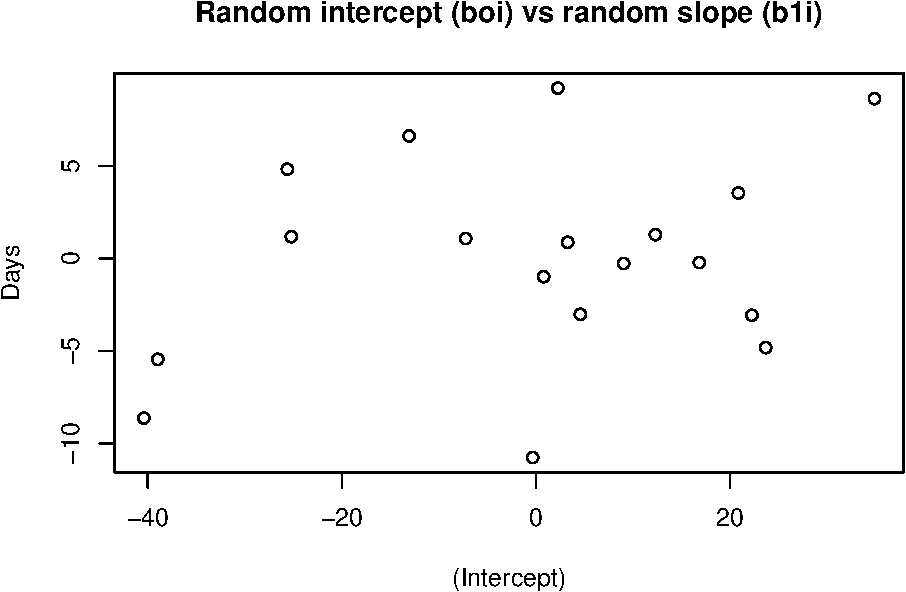
\includegraphics{Common_sleep_files/figure-latex/unnamed-chunk-8-1.pdf}

\begin{verbatim}
##     (Intercept)      Days
## 308    253.6626 19.666560
## 309    211.0108  1.846770
## 310    212.4488  5.017706
## 330    275.0940  5.653141
## 331    273.6636  7.397609
## 332    260.4439 10.195232
\end{verbatim}

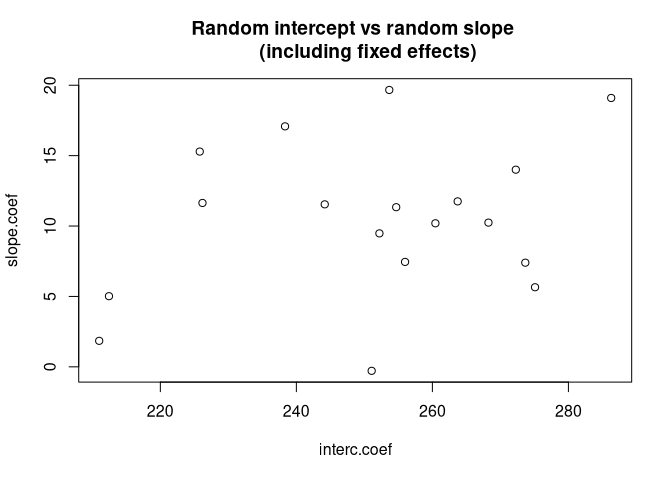
\includegraphics{Common_sleep_files/figure-latex/unnamed-chunk-8-2.pdf}
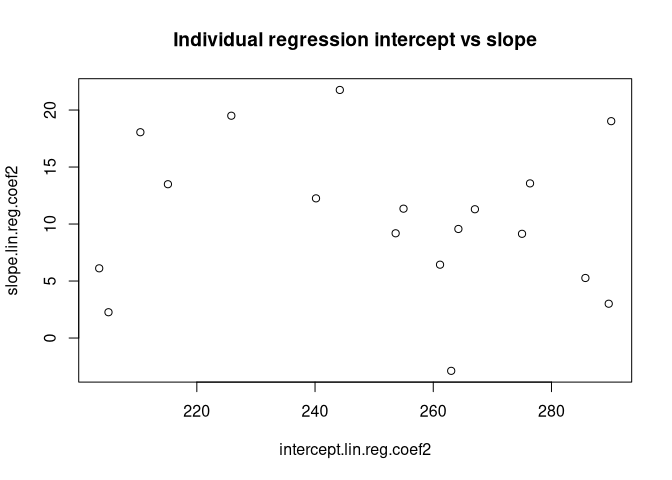
\includegraphics{Common_sleep_files/figure-latex/unnamed-chunk-8-3.pdf}
\#\#\# to do: compare the two models by creating the mean!

\end{document}
